%!TEX root = ../document.tex

\section[Point of View (Author: Felix Leupold)]{Point of View} \label{sec:POINT_OF_VIEW}

A point of view (POV) consists of three parts: a concrete specification of the user we are designing for, his or her needs we are trying to satisfy with our solution and finally an insight we derived from the understanding and observation phase. We present all of these in this section.

We derive a \emph{"How might we..."}-question from our POV and try to answer this question during the ideation phase. This description presents our final Persona and her needs. Throughout the course we repeatedly adapted our Persona slightly as we discovered new needs and reevaluated their importance for our persona.

\subsection{Persona}
\label{subsec:persona}

Our Persona is Amber, she is 31 years old and for roughly six years has she been working as a Software Developer at a big company that use HANA as a database for their applications. Within her team of ten developers, she programs applications that work on big data sets and are performance critical. While her main focus is on the backend side, she does not consider herself a database expert. Though she still knows how to write SQL queries, she is not able to predict the impact of certain changes in a query formulation on its performance just by looking at the statement. She works in her favorite development environment studio, which is Eclipse\footnote{\url{http://www.eclipse.org/}}. As a seperate environment, HANA Studio allows her to look at the content or schema of the database.

Amber enjoys coding a lot. It is the favorite part of her work. She is also very enthusiastic and wants to get features completed as fast as possible. She uses a lot of different tools that help her simplify reoccurring tasks and boost her productivity.

However, throughout her work day Amber usually experiences a lot of interruptions. We refer to these interruptions as \emph{Context Switches} that pull her out of her workflow. These might be small switches, like changing from the editor to the browser to browse for something online but can also be bigger ones, such as having to write an email or even physical interruptions caused by colleagues who ask for her attention.

\begin{figure}
    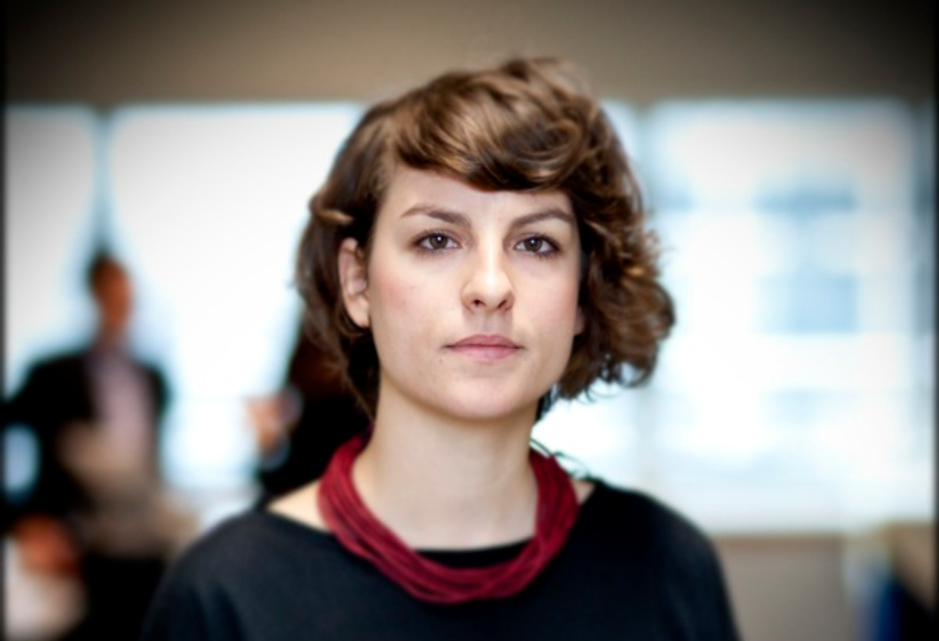
\includegraphics[width=\linewidth]{images/amber}
    \caption{Our Persona Amber, a software developer for performance critical big data applications.}
    % #selfrespect
    \label{fig:amber}
\end{figure}

\subsection{Needs}
Amber's needs are manyfold. The essential ones are:

\begin{itemize}
	\item She wants to do her work in the most efficient way.
	\item Since her applications are performance critical, she needs to evaluate her code against real customer data.
	\item Amber is not an SQL expert. Thus, she needs a way to explore and learn which parts of a query perform well and where bottlenecks are.
	\item She wants her productivity tool chain to be integrated into her IDE in order to avoid switching contexts.
	\item The general number of Context Switches needs to be minimized.
\end{itemize}

Throughout the seminar we down-weighted the importance of the last point as we narrowed down the interruptions that we wanted to tackle. We discovered that although big Context Switches like replying to emails lead to longer disruptions, they occur way less frequently than small Context Switches, such as navigating between applications. Thus tackling issues of the latter type may, accumulated, lead to a big increase in efficiency which is why we focused on that.

\subsection{Insight}

During our observations we saw how our Persona figured out to understand SQL queries written in code. She copied the query from her Eclipse editor into HANA Studio. As in Eclipse her query appears as multiple split \emph{Strings} she has to escape all contained quotes. This is the first Context Switch. Most queries also contain parameters that are bound during runtime. In order to execute the query in HANA Studio Amber looks up appropriate values in the schema. This is the second Context Switch. If the executed query does not behave as expected she is forced to go over this whole process again, switching back and forth in the Studio between edit- and result-view mode. There is no way to recognize the impact of query changes on the result in the same window. Thus, this results in a number of additional Context Switches. If the query finally behaves as desired, Amber has to copy it back into her code editor and turn all concrete values back into variables.

We consider this interaction as a workaround and take it as a foundation for our Point Of View as it emphasizes the most important need. That is predicting the impact of queries on the underlying data. We combine our Persona and her need with one of the insights we gathered during our interviews, namely that \textit{Code needs data context} (cf. Section \ref{sec:OBSERVE}).


\subsection{POV Statement}

\begin{description}
	\item [User] Amber, a productivity junkie, working with HANA on performance critical big data business applications.
	\item [Need] Amber needs to predict the performance and logical impact of her code on the underlying data sets using only without switching to another application.
	\item [Insight] Code needs data context.
\end{description}

Based on this, we derived the following \emph{"How might we question..."}:

\subsection{How Might We...}

\begin{quote}
\emph{"How might we help Amber to predict the impact of her code on real customer data in one integrated development environment?"}
\end{quote}